\documentclass{sig-alternate}

\usepackage[utf8]{inputenc}
\usepackage[T1]{fontenc}
\usepackage{graphicx}
\usepackage{amssymb}
\usepackage{amsmath}
\usepackage{mysymbols}
\usepackage{hyperref}
\usepackage{tikz}

\newtheorem{definition}{Definition}
\newtheorem{theorem}[definition]{Theorem}
\newtheorem{lemma}[definition]{Lemma}
\newtheorem{corollary}[definition]{Corollary}
\newtheorem{proposition}[definition]{Proposition}

\usepackage{algorithm}
\usepackage{algorithmic}
\renewcommand{\algorithmicrequire}{\textbf{Input:}}
\renewcommand{\algorithmicensure}{\textbf{Output:}}

\usepackage{xcolor}
\newcommand{\todo}[1]{\textcolor{red}{(#1)}}

\newcommand{\Cyc}{\Phi}  % Cyclotomic polynomial
\newcommand{\bb}{\mathbf{B}}  
\newcommand{\uu}{\mathbf{U}}  % bases for lift and push

\newdef{remark}{Remark}

\begin{document}

\title{Cool title to catch Lenstra's eye goes here}
\numberofauthors{3}
\author{
  \alignauthor Luca De Feo
  \alignauthor Javad Doliskani
  \alignauthor \'Eric Schost
}

\maketitle
\begin{abstract}
  We build towers.
\end{abstract}
\category{F.2.1}{Theory of computation}{Analysis of algorithms and problem complexity}[Computations in finite fields]
\category{G.4}{Mathematics of computing}{Mathematical software}
\terms{Algorithms,Theory}
\keywords{Finite fields, irreducible polynomials, extension towers, algebraic tori, elliptic curves.}

%%%

\section{Introduction}
\label{sec:intro}

Building arbitrary finite extensions of finite fields is a fundamental
task in any computer algebra system. Many systems are limited to
construct extensions of prime fields, but there is one notable
exception: Magma~\cite{MAGMA} has implemented for a long time a
powerful system of ``compatibly embedded finite
fields''~\cite{bosma+cannon+steel97}, capable of building extensions
of any finite field and taking track of the embeddings between the
fields.

The system implemented in Magma, as described in the original paper,
uses linear algebra to describe the embeddings of finite fields. From
a complexity point of view, this is far from optimal: one may hope to
compute and apply the morphisms in (quasi)-linear time in the degree
of the extension, but this is usually out of reach of plain linear
algebra techniques. Even worse, the quadratic memory requirements make
the system unsuitable for embeddings of large degree
extensions. Although the Magma core has evolved since the publication
of the paper, experiments in Section~\ref{sec:impl} show that
embeddings of large extension fields are still out of reach.

In this paper, we discuss an approach based on polynomial arithmetic
rather than linear algebra, yielding much better performances. We only
consider some special cases, but we expect that these results will
pave the way towards a complete solution.

%% The families of polynomials we use come from work of
%% Shoup~\cite{Shoup90,shoup94} and Couveignes and Lercier on
%% constructing irreducible polynomials~\cite{couveignes+lercier11}, as
%% well as Lenstra and De Smit on the algebraic closure of finite
%% fields~\cite{lenstra+desmit08-stdmodels}.

Let $q$ be a power of a prime $p$, let $\F_q$ be the finite field with
$q$ elements and let $\ell$ be a new integer. Our main interest in
this paper is on the algorithmic aspects of the \emph{$\ell$-adic
  closure} of $\F_q$, which is defined as follows. Fix arbitrary
embeddings
\begin{equation*}
  \F_q \subset \F_{q^\ell} \subset \F_{q^{\ell^2}} \subset \cdots;
\end{equation*}
then, the $\ell$-adic closure of $\F_q$ is the infinite field defined by
\begin{equation*}
  \F_q^{(\ell)} = \bigcup_{i\ge 0}\F_{q^{\ell^i}}.
\end{equation*}
We also call an \emph{$\ell$-adic tower} the sequence of extensions
$\F_q,\F_{q^\ell},\dots$ An important feature of $\ell$-adic towers is
that they allow us to build the algebraic closure $\bar{\F}_q$ of
$\F_q$, as there is an isomorphism
\begin{equation*}
  \label{eq:tensor}
  \bar{\F}_q \isom \bigotimes_{\ell\text{ prime}} \F_q^{(\ell)},
\end{equation*}
where the tensor products are over $\F_q$.

In this paper, we give algorithms that allow us to ``compute''
efficiently in the first levels of such $\ell$-adic towers, in a sense
defined hereafter.  We do not discuss the representation of the base
field $\F_q$ itself, and we count arithmetic operations
$\{+,-,\times,\div\}$ in $\F_q$ at unit cost. 

%% Since our focus is on the representation of extensions of large
%% degree, we do not consider issues related to special representations
%% of small finite fields, such as primitive polynomials, Zech
%% logarithms, Conway polynomials, etc.

The techniques we present are similar to those in~\cite{df+schost12}
in that we construct families of irreducible polynomials with special
properties, then give algorithms that exploit the special form of
those polynomials to apply the embeddings.

Each field $\F_{q^{\ell^i}}$ is represented as a univariate quotient ring
$\F_q[X_i]/\langle Q_i\rangle$, for some irreducible polynomial $Q_i
\in \F_q[X_i]$. Below, we will let $x_i$ be the residue class of $X_i$
modulo $Q_i$, so that $\F_{q^{\ell^i}}$ is endowed with the monomial
basis
\begin{equation}
  \label{eq:uni-basis1}
  \mathbf{U}_i = (1,x_{i},x_{i}^2,\ldots,x_{i}^{\ell^{i}-1}).
\end{equation}
Using this representation allows us to use asymptotically fast
algorithms for basic arithmetic operations. Let indeed $\Mult : \N
\rightarrow \N$ be such that polynomials in $\F_q[X]$ of degree less
than $n$ can be multiplied in $\Mult(n)$ operations in $\F_q$, under
the assumptions of~\cite[Ch.~8.3]{vzGG}; using FFT multiplication, one
can take $\Mult(n)=O(n\log (n) \log\log (n))$. Then, multiplications
and inversions in $\F_q[X_i]/\langle Q_i \rangle$ can be done in
respectively $O(\Mult(\ell^i))$ and $O(\Mult(\ell^i)\log(\ell^i))$
operations in $\F_q$~\cite[Ch.~9-11]{vzGG}. This is almost optimal, as
both results are quasi-linear in $[\F_{q^{\ell^i}}:\F_q]=\ell^i$.

Computing embeddings requires more work. For this problem, it is
enough consider a pair of consecutive levels in the tower; any other
embedding is done by applying repeatedly this elementary
operation. Following again~\cite{df+schost12}, we will introduce two
slightly more general operations, {\em lift} and {\em push}.

For $i \ge 0$, $\F_{q^{\ell^{i+1}}}$ has two natural representations
as a vector space over $\F_q$. The first one is via the monomial basis
$\mathbf{U}_{i+1}$ seen above, corresponding to the univariate model
$\F_q[X_{i+1}]/ \langle Q_{i+1} \rangle$. The second one amounts to
seeing $\F_{q^{\ell^{i+1}}}$ as a degree $\ell$ extension of
$\F_{q^{\ell^{i}}}$, that is, as
\begin{equation}\label{eq:QiTi}
\F_q[X_i,X_{i+1}]/\langle Q_i(X_i), T_i(X_i,X_{i+1})\rangle,  
\end{equation}
for some polynomial $T_i$ monic of degree $\ell$ in $X_{i+1}$, and of
degree less than $\ell^i$ in $X_i$.  The corresponding basis is
bivariate and involves $x_i$ and $x_{i+1}$:
\begin{equation}
  \label{eq:bi-basis}
  \mathbf{B}_{i+1} = (1,\ldots,x_i^{\ell^i-1},\ldots,x_{i+1}^{\ell-1},\ldots,x_i^{\ell^i-1}x_{i+1}^{\ell-1}).
\end{equation}
{\em Lifting} corresponds to the change of basis from
$\mathbf{B}_{i+1}$ to $\mathbf{U}_{i+1}$; {\em pushing} is the inverse
transformation.

Provided $Q_i$ and $T_i$ are known, lift and push allow us to perform
embeddings as a particular case, but they are also the key to many
further operations. We will not give details here and refer
to~\cite{df+schost12,DoSc12,LeSc12} for examples; we simply mention
the computation of relative traces, norms or characteristic
polynomials, as well as applications to solving Artin-Schreier
equations, or quadratic equations, given in~\cite{df+schost12,DoSc12}
for respectively $\ell=p$ and $\ell=2$.

The main results in this paper are efficient algorithms for building
the families of polynomials $Q_i$ and $T_i$, and for performing lift
and push operations. In all that follows, we exclude the cases
$\ell=p$ and $\ell=2$, which are dealt with
in~\cite{df+schost12,DoSc12}.

\paragraph*{\bf Previous work}
In~\cite{Shoup90,shoup94}, Shoup gives an algorithm for constructing
irreducible polynomials over $\F_q$ that follows the same pattern as
above: in order to build an irreducible polynomial of degree $n$, one
reduces to the case where $n$ is a power of a prime $\ell$, with
special treatments for the quadratic ($\ell=2$) and Artin-Schreier
cases ($\ell=p$).

Couveignes and Lercier give an alternative construction with
complexity subquadratic in $\ell$~\cite{couveignes+lercier11}; we will
discuss it in Section~\ref{sec:fibers}.


Most computer algebra systems construct the field $\F_q$ by taking
degree $d$ polynomials at random until one irreducible is found. This
approach has a cost at least quadratic in the degree $d$. More
advanced constructions use Eq.~\eqref{eq:tensor}: they factor $d$ into
prime powers, for each prime power construct an extension of $\F_p$ of
that degree, then glue all the extensions together by taking
\emph{composita}.

The classical way of taking \emph{composita} is \todo{where?}

\paragraph*{\bf Applications}
A variety of computations in number theory and algebraic geometry
requires frequently constructing new extension fields and moving
elements from one to the other. Examples of these algorithms
are~\cite{df10} \todo{cite more}. Our construction makes them feasible
for much larger sizes than it was previously possible.


%% For any $n \ge 1$, the field $\F_{q^n}$ can be constructed as the
%% splitting field of any irreducible polynomial of degree $n$ in
%% $\F_q[X]$. There are about $q^n/n$ such irreducible
%% polynomials~\cite[Corollary~7.\S2.2]{ireland1990classical}, giving as
%% many different ways of representing $\F_{q^d}$. There is no canonical
%% way of establishing isomorphisms between them, since a field with
%% $q^n$ elements has $n$ automorphisms fixing $\F_q$. For the same
%% reasons, when $n$ divides $n'$, there is no canonical embedding 
%% of $\F_{q^n}$ into $\F_{q^{n'}}$.

If $L/K$ is a field extension, we write $\Tr_{L/K}$, $\Norm_{L/K}$ and
$\Gal_{L/K}$ for the trace, the norm and the Galois group of the
extension, respectively. When the field $L$ is clear from the context,
we simply write $\Tr_K$ and $\Norm_K$, and when the field $K$ is clear
too, we may write $\Tr$ and $\Norm$.

%%%%%%%%%%%%%%%%%%%%%%%%%%%%%%%%%%%%%%%%%%%%%%%%%%%%%%%%%%%%
%%%%%%%%%%%%%%%%%%%%%%%%%%%%%%%%%%%%%%%%%%%%%%%%%%%%%%%%%%%%
%%%%%%%%%%%%%%%%%%%%%%%%%%%%%%%%%%%%%%%%%%%%%%%%%%%%%%%%%%%%

\section{XXX's towers}
\label{sec:LDtower}

Let $\ell,p$ be odd primes, with $\ell \ne p$, and let $q$ be a power
of $p$. In this section, we discuss a construction of the $\ell$-adic
tower over $\F_q$ inspired by previous work of
Shoup~\cite{Shoup90,shoup94}, Lenstra-De
Smit~\cite{lenstra+desmit08-stdmodels} and
Couveignes-Lercier~\cite{couveignes+lercier11}.

We start by constructing an extension $\K_0 = \F_q[Y_0]/\langle P_0
\rangle$, such that the residue class $y_0$ of $Y_0$ is a non
$\ell$-adic residue in $\K_0$ (we discuss this in more detail in the
first subsection), and we let $r$ be the degree of $P_0$.

By~\cite[Th.~VI.9.1]{lang}, for $i\ge 1$, the polynomial
$Y_i^{\ell^i}-y_0$ is irreducible in $\K_0[Y_i]$, so that $\K_i=
\K_0[Y_i]/\langle Y_i^{\ell^i}-y_0\rangle$ is a field with $q^{r
  \ell^i}$ elements.  If we let $y_i$ be the residue class of $Y_i$ in
$\K_i$, these fields are naturally embedded in one another by the
isomorphism $\K_{i+1} \simeq \K_i[Y_{i+1}]/\langle
Y_{i+1}^\ell-y_i\rangle$; in particular, the relation
$y_{i+1}^\ell=y_i$ holds.

In order to build $\F_{q^{\ell^i}}$, we apply a descent process, for
which we follow~\cite[Th.~2.1]{Shoup90}. For $i \ge 0$, let $x_i$ be
the trace of $y_i$ over a subfield of index $r$:
\begin{equation}\label{eq-def:xi}
x_i = \sum_{j = 0}^{r-1} y_i^{q^{\ell^i j}}.  
\end{equation}
Then, the reference above proves that
$\F_q(x_i)=\F_{q^{\ell^i}}$, so that the minimal polynomials
 of $x_1,x_2,\dots$ for the family of irreducible polynomials
$Q_i$ we are interested in. This situation is depicted in
Figure~\ref{fig:ladic}.

\begin{figure}[h]
  \centering
  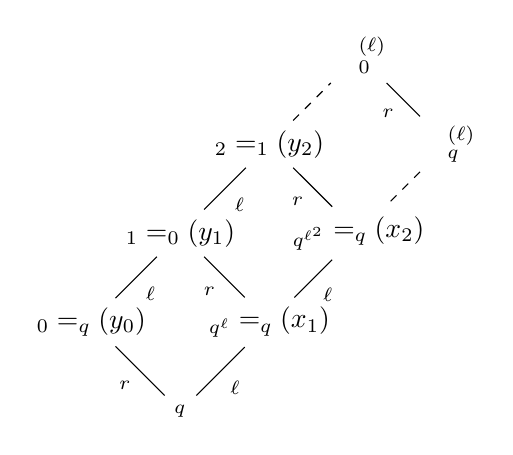
\begin{tikzpicture}[node distance=1.6cm]
    \node(Q){$\F_q$};
    \node(Q0)[above left of=Q]{$\K_0=\F_q(y_0)$};
    \node(K1)[above right of=Q]{$\F_{q^\ell}=\F_q(x_1)$};
    \node(Q1)[above right of=Q0]{$\K_1=\K_0(y_1)$};
    \node(K2)[above right of=K1]{$\F_{q^{\ell^2}}=\F_q(x_2)$};
    \node(Q2)[above right of=Q1]{$\K_2=\K_1(y_2)$};
    \node(Koo)[above right of=K2]{$\quad \F_q^{(\ell)}$};
    \node(Qoo)[above right of=Q2]{$\quad\K_0^{(\ell)}$};
    \draw (Q) edge node[auto]{\scriptsize$r$} (Q0)
              edge node[auto,swap]{\scriptsize$\ell$} (K1)
          (K1) edge node[auto]{\scriptsize$r$} (Q1)
               edge node[auto,swap]{\scriptsize$\ell$} (K2)
          (Q1) edge node[auto]{\scriptsize$\ell$} (Q0)
          (Q2) edge node[auto,swap]{\scriptsize$r$} (K2)
               edge node[auto]{\scriptsize$\ell$} (Q1)
               edge[dashed] (Qoo)
          (Koo) edge[dashed] (K2)
               edge node[auto]{\scriptsize$r$} (Qoo);
  \end{tikzpicture}
  \caption{The $\ell$-adic towers over $\F_q$ and $\K_0$.}
  \label{fig:ladic}
\end{figure}

In this section, we show how to compute the polynomials $Q_i$, the
polynomials $T_i$ introduced in Eq.~\eqref{eq:QiTi} and how to perform
lift and push. We will actually consider more general minimal
polynomials: for $0 \le j < i$, we will let $Q_{i,j} \in
\F_q(x_j)[X_j]$ be the minimal polynomial of $x_i$ over $\F_q(x_j)$,
so that $Q_{i,j}$ has degree $\ell^{i-j}$, with in particular
$Q_{i,0}=Q_i$ and $Q_{i,i-1}=T_{i-1}(x_{i-1},X_i)$.

We first explain the initialization of the process (computing
$P_0$). Then, we consider two favorable cases, where $\ell$ divides
respectively $q-1$ and $q+1$, and finally discuss the general case.


%%%%%%%%%%%%%%%%%%%%%%%%%%%%%%%%%%%%%%%%%%%%%%%%%%%%%%%%%%%%

\subsection{Finding $P_0$}

To determine $P_0$, two constructions will be used. In both cases, we
start from the $\ell$-th cyclotomic polynomial $\Cyc_\ell \in
\Z[X_0]$. The first step consists in factoring $\Cyc_\ell$ over
$\F_q[X_0]$: by~\cite[XXX]{shoup94}, this takes an expected $O(\dots)$
operations in $\F_q$.

Over $\F_q[X_0]$, $\Cyc_\ell$ splits into irreducible factors of the
same degree $r$, where $r$ is the order of $q$ in $\Z/\ell\Z$ (so $r$
divides $\ell-1$); let $F_0$ be one of these factors. By construction,
there exist non $\ell$-adic residues in $\F_q[X_0]/\langle F_0
\rangle$. Once such a non-residue $\eta$ is found, we simply let $P_0$
be its minimal polynomial over $\F_q$ (which still has degree $r$);
given $\eta$, computing $P_0$ takes $O(\dots)$ operations in $\F_q$.

To find $\eta$, Shoup's approach consists in picking it at random: we
expect to find a non $\ell$-adic residue after an expected $O(1)$
trials, and each trial takes $O(\dots)$ operations in $\F_q$.

An alternative, proposed by Lenstra and De Smit, is to take iterated
$\ell$-th roots of $X_0 \bmod F_0$ until we find a non-residue. As
stated in~\cite{lenstra+desmit08-stdmodels}, this requires to take
$\kappa$ successive $\ell$-th roots modulo $F_0$ until hitting a
non-residue $\eta$, where $\kappa$ is the $\ell$-adic valuation of
$(q^{\ell-1}-1)/\ell$. Note that in this case, $\eta$ is a root of
unity of order $\ell^{\kappa+1}$.

%%%%%%%%%%%%%%%%%%%%%%%%%%%%%%%%%%%%%%%%%%%%%%%%%%%%%%%%%%%%

\subsection{$T_1$-type extensions}\label{ssec:T1}

In this subsection, we consider the simplest case, where $\ell$
divides $q-1$. In this case, $\Phi_\ell$ splits into linear factors
over $\F_q$ (that is, $r=1$). The polynomial $P_0$ is of the form
$Y_0-\eta$, where $\eta$ is a non $\ell$-adic residue in $\F_q$. In
this case, we simply find $\eta$ by random trial in $\F_q$, as no gain
is to be found from the more specific choice used by Lenstra-De Smit.

In this situation, no descent is required. For $i \ge 0$, we have
$\K_i=\F_{q^{\ell^i}}$ and $x_i=y_i$; the families of polynomials we
obtain are
$$Q_i=X_i^{\ell^i}-\eta \quad\text{and}\quad T_i=X_{i+1}^\ell-X_i.$$
Lifting amounts to taking $F = \sum_{0 \le j < \ell^{i+1}} f_j
x_{i+1}^j$ and rewriting it as a bivariate polynomial in
$x_i,x_{i+1}$, using the rule
$$x_{i+1}^j = x_i^{\,j {\rm~div~} \ell} x_{i+1}^{\,j \bmod \ell}.$$
Pushing does the converse operation, using the rule
$$x_i^e x_{i+1}^f = x_{i+1}^{e \ell + f}.$$ Thus, both operations
involve only exponent arithmetic, and no operation in $\F_q$.

%%%%%%%%%%%%%%%%%%%%%%%%%%%%%%%%%%%%%%%%%%%%%%%%%%%%%%%%%%%%

\subsection{$T_2$-type extensions}

Next, we consider the case where $\ell$ divides $q+1$, so that
$\Phi_\ell$ splits into quadratic factors over $\F_q$ (that is,
$r=2$). In this case, we use Lenstra and De Smit's construction of
$P_0$; it leads in particular to the following useful property.

\begin{lemma}
  For $i \ge 0$, $x_i = y_i +y_i^{-1}$.
\end{lemma}
\begin{proof}
  By definition, $x_i=y_i+y^{q^{\ell^i}}$. Recall that in the
  Lenstra-De Smit construction, $y_0$ has order $\ell^{\kappa+1}$,
  where $\kappa$ is the $\ell$-adic valuation of
  $(q^{\ell-1}-1)/\ell$. Thus, $y_i$ has order $\ell^{i+\kappa+1}$, so
  to conclude, it is enough to prove that $\ell^{i+\kappa+1}$ divides
  $q^{\ell^i}+1$.

  Because $\ell$ divides $q+1$, a quick induction shows that $q+1$ and
  $q^{2n}-1$ have the same $\ell$-adic valuation, for all positive
  integers $n$. In particular, $\kappa$ is the $\ell$-adic valuation
  of $(q+1)/\ell$, so that $\ell^{\kappa+1}$ divides $q+1$, and another
  induction on $i$ finishes the proof of the lemma.
\end{proof}


\begin{corollary}
  For $1 \le j < i$, $Q_{i,j} \in \F_q(x_{j})[X_i]$ satisfies
  \begin{equation*}
    \label{eq:T2-relpols}
    Q_{i,j}(X_i)^2 = \mathrm{Res}_{Y_i}(Y_i^{2\ell^j}-x_{j}Y_i^{\ell^j}+1,\; Y_i^2-X_i Y_i+1).
  \end{equation*}
\end{corollary}
\begin{proof}
  The previous lemma shows that the minimal polynomial of $y_i$ over
  $\F_q(x_i)$ is $Y_i^2 -x_i Y_i +1$. By composition, it follows that
  the minimal polynomial of $y_i$ over $\F_q(x_{j})$ is
  $Y_i^{2\ell^j}-x_{j} Y_i^{\ell^j}+1$. Eliminating $Y_i$ between
  these two polynomials will give the required relation between
  $x_{j}$ and $x_i$. Explicitly, the resultant above 
  is equal to
\begin{align*}
   \prod_{\sigma\in\Gal_{\K_i/\F_q(x_{j})}}
  (y_i^2 - X_i y_i + 1)^\sigma \\
  % 
  =\Norm_{\K_i/\F_q(x_{j})}(y_i) \prod_{\sigma\in\Gal_{\K_i/\F_q(x_{j})}} 
  (y_i + y_i^{-1} - X_i)^\sigma \\
  % 
  =\left(\prod_{\sigma\in\Gal_{\K_i/\F_q(x_{j})}/\langle\tau\rangle}
    (x_i - X_i)^\sigma\right)^2 \\
  % 
  =\left(\prod_{\sigma\in\Gal_{\F_q(x_i)/\F_q(x_{j})}}
    (x_i - X_i)^\sigma\right)^2 =Q_{i,j}(X_i)^2,
\end{align*}
where the third equality is true because
$\Norm_{\K_i/\F_q(x_{j})}(y_i)=1$, as seen from the minimal polynomial of
$y_i$, and where $\tau$ is the element of
$\Gal_{\K_i/\F_q(x_{j})}$ such that $\tau:y_i\mapsto y_i^{-1}$.
\end{proof}

As evident from the formula, given a field $\K$ and $z \in \K$, we
just need to show how to compute
\begin{equation*}
  Q(X) = \sqrt{\mathrm{Res}_Y(Y^{2 n}-z Y^n+1, Y^2-XY+1)}.
\end{equation*}
Let $\zeta$ and $\zeta^{-1}$ be the two roots of $Y^2-XY+1$ over an
algebraic closure of $\K(X)$. By a direct calculation, we find
\begin{equation*}
  Q(X) = \zeta^n + \zeta^{-n} - z.
\end{equation*}
As a result, $Q$ can be computed in $O(\Mult(n))$ operations in $\K$,
using repeated squaring modulo $Y^2-XY+1$. In particular, taking
$n=\ell^i$ and returning to our initial problem, $Q_i$ can be computed
in time $O(\Mult(\ell^i))$. Taking $n=\ell$, we see that the
polynomials $T_i$ all take the same form, and each of them can be
computed in time $O(\Mult(\ell))$.

We now present a better solution, valid in large enough
characteristic. For $n \in \N$, the term $P_{n}=\zeta^{n} +
\zeta^{-n}$ is the $n$-th power sum of $Y^2-XY+1$, thus, using
Newton's identities,
\begin{equation}
  \label{eq:simple}
  \begin{aligned}
    P_0 &= 2,\\
    P_1 &= X,\\
    P_{n+1} &= X P_{n} - P_{n-1}.
  \end{aligned}
\end{equation}
Writing $P_n = \sum_i c_{n,i}X^{n-i}$, we deduce the relation
\begin{equation}
  c_{n,i} = c_{n-1,i} - c_{n-2,i-2}.
\end{equation}
%% We arrange these coefficients like in Pascal's triangle:
%% \begin{equation}
%%   \begin{tabular}{*{8}{c@{}}}
%%     &&&2\\
%%     &&1&&0\\
%%     &1&&0&&-2\\
%%     1&&0&&-3&&0
%%   \end{tabular}
%% \end{equation}
%% It is then evident that every second column is identically zero, and
%% that signs alternate in odd columns. 
Removing the odd values of $i$ and taking absolute values, i.e.,
setting $b_{n,k}=\lvert c_{n+k,2k}\rvert$, the new coefficients
satisfy the relation
\begin{equation*}
  b_{n,k} = b_{n-1,k} + b_{n-1,k-1},
\end{equation*}
which is the same as Pascal's relation. Indeed, we obtain the
$(1,2)$-Pascal triangle, also called Lucas'
triangle~\cite{benjamin10}:
\begin{equation*}
  \begin{tabular}{*{8}{c@{}}}
    &&&2\\
    &&1&&2\\
    &1&&3&&2\\
    1&&4&&5&&2
  \end{tabular}
\end{equation*}
A special case of this fact was already proven by Gauss, and the
general proof is in~\cite[Prop.~1]{gurak06}. It is well known that
the coefficients of Lucas' triangle are related to those of Pascal's
by
\begin{equation}
  \label{eq:lucas-tri}
  b_{n,k} = \binom{n}{k} + \binom{n-1}{k-1} = \frac{n+k}{n}\binom{n}{k}.
\end{equation}
By using Eq.~\eqref{eq:lucas-tri} and the sign alternation property,
we obtain 
\begin{gather}
  c_{n,2k} = (-1)^kb_{n-k,k} = (-1)^k\frac{n}{n-k}\binom{n-k}{k},\\
  \label{eq:lucas-recurrence}
  \frac{c_{n,2k+2}}{c_{n,2k}} = 
  -\frac{(n-2k)(n-2k-1)}{(n-k-1)(k+1)}.
\end{gather}
Provided all denominators are invertible,
Eq.~\eqref{eq:lucas-recurrence} gives a formula to compute all the
coefficients of $Q_{i}$ using $O(\ell^{i})$ operations in $\F_p$, and
gives similarly the coefficients of $T_i$ in $O(\ell)$ operations.

%% Eq.~\eqref{eq:lucas-recurrence} gives a formula to compute all the
%% coefficients of $Q_{i,j}$ using $O(\ell^{j-i})$ operations in $\F_p$. By
%% performing the same computation in the ring of $p$-adic integers with
%% just one digit of floating precision, it is possible to compute
%% $Q_{i,j}\bmod p$ using $O(\ell)$ operations in $\F_p$.

%% One remarkable property of the Lucas triangle is that the
%% anti-diagonals sum up to the Lucas numbers:
%% \begin{equation}
%%   \sum_{k\ge0} b_{n-k,k} = \sum_{k\ge0} \lvert c_{n,2k}\rvert = L_n.
%% \end{equation}
%% A funny consequence of this property is the following equality on
%% complex numbers
%% \begin{equation}
%%   \label{eq:lucas-fun}
%%   p_\ell(i) = \sum_{k\ge0} c_{\ell,k}i^{\ell-k} = i^\ell L_\ell.
%% \end{equation}

%%%%%%%%%%%%%%%%%%%%%%%%%%%%%%%%%%%%%%%%%%%%%%%%%%%%%%%%%%%%

\subsection{The general case}

Finally, we discuss the general situation, where we do not make any
assumption on the behavior of $\Phi_\ell$ in $\F_q[X]$.  Since we are
not able to exploit the more specific Lenstra-De Smit construction in
this case, we use Shoup's approach, picking the initial non
$\ell$-adic residue $\eta$ at random.

Because $r=[\K_0 : \F_q]$ divides $\ell-1$, it is coprime with
$\ell$. Thus, $Q_i$ remains the minimal polynomial of $x_i$ over
$\K_0$, and more generally $Q_{i,j}$ remains the minimal polynomial of
$x_i$ over $\K_{j}$; this will allow us to replace $\F_q$ by $\K_0$ as
our base field. We will measure all costs by counting operations in
$\K_0$, and we will deduce the cost over $\F_q$ by adding a factor
$O(\Mult(r)\log(r))$ to account for the cost of arithmetic in $\K_0$.

For $i \ge 0$, since $\K_i=\K_0[Y_i]/\langle Y_i^{\ell^i}-y_0\rangle$,
we represent the elements of $\K_i$ on the basis $\{y_i^e \mid 0 \le e
< \ell^i\}$; then, all arithmetic operations in $\K_i$ can be done in
$O(\Mult(\ell^i)\log(\ell^i))$ operations in $\K_0$. Note that $x_i$
is written on this basis as
\begin{equation}\label{eq-def:xiyi}
x_i = \sum_{j = 0}^{r-1} y_i^{q^{\ell^i j} \bmod \ell^i}
y_0^{q^{\ell^i j} {\rm~div~} \ell^i}. 
\end{equation}

Our strategy is to show how to convert between two univariate bases of
$\K_i$, $\{y_i^e \mid 0 \le e < \ell^i\}$ and $\{x_i^e \mid 0 \le e <
\ell^i\}$. In other words, we show how to apply the isomorphism
$$\Psi_i: \K_i=\K_0[Y_i]/\langle Y_i^{\ell^i}-y_0\rangle \to
\K_0[X_i]/\langle Q_{i,0}\rangle$$ and its inverse; we will compute
the required polynomials $Q_{i,0}$ and $Q_{i,i-1}$ as a byproduct. In
a second time, we will use $\Psi_i$ to perform push and lift between
the monomial basis in $x_i$ and the bivariate basis in
$(x_{i-1},x_i)$.

We proceed step-by-step, factoring $\Psi_i$ into elementary
isomorphisms
$$\Psi_{i,j}: \K_j[X_i]/\langle Q_{i,j}\rangle \to
\K_{j-1}[X_i]/\langle Q_{i,j-1}\rangle,$$ for $j=i,\dots,1$.  To start
the process, with $j=i$, we let $Q_{i,i}=X_i-x_i \in \K_i[X_i]$,
so that $\K_i=\K_i[X_i]/\langle Q_{i,i} \rangle$.

Let $j \le i$ and suppose that $Q_{i,j}$ is known. We are going to
factor $\Psi_{i,j}$ further as $\Phi''_{i,j} \circ \Phi'_{i,j} \circ
\Phi_{i,j}$. First, we introduce the isomorphism
$$\varphi_j: \K_j \to \K_{j-1}[Y_j]/\langle Y_j^\ell-y_{j-1}\rangle.$$
The forward direction is a push from the monomial basis in $y_j$ to
the bivariate basis in $(y_{j-1},y_j)$ and the inverse is a lift; none
of them involves any arithmetic operation, as was pointed out in
Subsection~\ref{ssec:T1}.  Then, we deduce the isomorphism
$$\Phi_{i,j}: \K_j[X_i]/\langle Q_{i,j} \rangle \to
\K_{j-1}[Y_j,X_i]/\langle Y_j^\ell-y_{j-1}, Q^\star_{i,j}\rangle,$$
where $Q^\star_{i,j}$ is obtained by applying $\varphi_j$ to all
coefficients of $Q_{i,j}$. Since $\Phi_{i,j}$ consists in a
coefficient-wise application of $\varphi_j$, applying it or its
inverse costs no arithmetic operations.

Next, changing the order of the variables $Y_j$ and $X_i$, we deduce
that there exists $S_{i,j}$ in $\K_{j-1}[X_j]$ such that we have an
isomorphism
\begin{multline*}
\Phi'_{i,j}: \K_{j-1}[Y_j,X_i]/\langle Y_j^\ell-y_{j-1}, Q^\star_{i,j}\rangle
\to\\ \K_{j-1}[X_i, Y_j]/\langle Q_{i,j-1}, Y_j-S_{i,j}\rangle;
\end{multline*}
where $\deg(Q^\star_{i,j},X_i)=\ell^{i-j}$ and
$\deg(Q_{i,j-1},X_i)=\ell^{i-j+1}$. This conversion is less obvious
than the previous one.
\begin{lemma}
  Given $Q^\star_{i,j}$, one can compute $Q_{i,j-1}$ and $S_{i,j}$
  using $O(\Mult(\ell^{i+1})\log(\ell))$ operations in $\K_0$.
  Once this is done, we can apply $\Phi'_{i,j}$ and its inverse 
  using $O(\Mult(\ell^{i+1}))$ operations in $\K_0$.
\end{lemma}
\begin{proof}
  We obtain $Q_{i,j-1}$ and $S_{i,j}$ from the resultant and degree-1
  subresultant of $Y_j-y_{j-1}$ and $Q^\star_{i,j}$ with respect to
  $Y_j$, computed over the polynomial ring $\K_{j-1}[X_i]$. This is
  done using Reischert's algorithm~\cite{Reischert97}. The direct
  analysis would yield a cost of
  $O(\Mult(\ell^{j-1})\Mult(\ell)\Mult(\ell^{i-j+1})\log(\ell))$
  operations in $\K_0$, accounting for respectively the cost of
  arithmetic in $\K_{j-1}$, the cost of the half-gcd algorithm in
  $Y_j$, and the cost of polynomial arithmetic in $X_i$. Using
  Kronecker's substitution to reduce all operations to trivariate
  arithmetic in $Y_{j-1},Y_j,X_i$ yields the claimed bound.

  Applying $\Phi'_{i,j}$ amounts to taking a polynomial $A(Y_j,X_i)$ 
  reduced modulo $\langle Y_j^\ell-y_{j-1}, Q^\star_{i,j}\rangle$
  and reducing it modulo $\langle Q_{i,j-1}, Y_j-S_{i,j}\rangle$. This
  is done by evaluating $Y_j$ at $S_{i,j}$, doing all operations
  modulo $Q_{i,j-1}$. Using Horner's scheme, this takes $O(\ell)$ 
  operations $(+,\times)$ in $\K_{j-1}[X_i]/\langle Q_{i,j-1}\rangle$,
  so the complexity claim follows.

  In the converse direction, we start from $A(X_i)$ reduced modulo
  $Q_{i,j-1}$; we have to reduce it modulo $\langle Y_j^\ell-y_{j-1},
  Q^\star_{i,j}\rangle$. This is done by applying the fast Euclidean
  division algorithm with coefficients in $\K_{j-1}[Y_j]/\langle
  Y_j^\ell-y_{j-1}\rangle$, for a cost of $O(\Mult(\ell^{i+1}))$
  operations in $\K_0$.
\end{proof}

The last isomorphism $\Phi''_{i,j}$ is trivial:
$$\Phi''_{i,j}: \K_{j-1}[X_i, Y_j]/\langle Q_{i,j-1}, Y_j-S_{i,j}\rangle
\to \K_{j-1}[X_i]/\langle Q_{i,j-1}\rangle$$
forgets the variable $Y_j$; it requires no arithmetic operation.

\medskip

Taking $j=i,\dots,1$ allows us to compute $Q_{i,i-1}$ and $Q_{i,0}$
for $O(i\Mult(\ell^{i+1})\log(\ell))$ operations in $\K_0$. Composing
the maps $\Psi_{i,j}$, we deduce further that we can apply $\Psi_i$ or
its inverse for $O(i\Mult(\ell^{i+1}))$ operations in $\K_0$.  

We claim that we can then perform push and lift between the monomial
basis in $x_i$ and the bivariate basis in $(x_{i-1},x_i)$ for the same
cost. Let us for instance explain how to lift.

We start from $A$ written on the bivariate basis in $(x_{i-1},x_i)$;
that is, $A$ is in $\K_0[X_{i-1},X_i]/\langle Q_{i-1},
T_{i-1}\rangle$. Apply $\Psi_{i-1}$ to its coefficients in
$x_i^0,\dots,x_i^{\ell-1}$, so as to rewrite $A$ as an element of
$$\K_0[Y_{i-1},X_i]/\langle Y_{i-1}^{\ell^{i-1}}-y_{i-2},
T_{i-1}\rangle = \K_{i-1}[X_i]/\langle Q_{i,i-1} \rangle.$$ Applying
$\Psi_{i,i}^{-1}$ gives us the image of $A$ in $\K_i$, and applying
$\Psi_i$ finally brings it to $\K_0[X_i]/\langle Q_{i}\rangle$.


%%%

\section{Towers from irreducible fibers}
\label{sec:fibers}
Every tower obtained by the Lenstra-De Smit construction, as well as
many others, can be understood in a geometrical way using an intuition
of Couveignes and Lercier\cite{couveignes+lercier11}. Suppose we are
given algebraic groups $G/\F_q$, $G'/\F_q$ and a degree $\ell$ map
$\phi:G'\to G$ surjective over the algebraic closure. If $\phi$ is not
surjective over $\F_q$, then some points of $G'$ will have fibers
consisting of $\ell$ distinct points of $G$ living in an algebraic
extension of $\F_q$. If $\phi$ is chosen well enough, these fibers can
be made to be irreducible over $\F_q$, so that an annihilating
polynomial will be irreducible of degree $\ell$, as required. If the
construction can be repeated with a new map $\phi':G''\to G'$, and so
on, then one is able to construct a tower of extensions of degree
$\ell$, ultimately leading to an $\ell$-adic closure. We now show how
this idea applies to the two examples shown before, then how
Couveignes and Lercier apply it to elliptic curves.

\paragraph{Algebraic tori}
In the case where $\ell$ divides $q-1$, the algebraic group involved
is the multiplicative group $\mathbb{G}_m/\F_q$, and the map is the
$\ell$-th power map defined by $\phi:x\mapsto x^\ell$. Since the map
is an endomorphism of $\mathbb{G}_m$, it can be iterated, yielding
each of the $\ell^i$-th power maps. It is well known, then, that if
$\zeta$ is a non $\ell$-adic residue, the polynomials
$X^{\ell^i}-\zeta$ corresponding to the fibers of $\phi^i$ are
irreducible over $\F_q$.

The case where $\ell$ divides $q+1$ is more interesting. Now
$\F_q(\zeta_i)$ is a quadratic extension of $\F_q(\eta_i)$. The
multiplicative subgroup defined by
\begin{equation}
  \label{eq:T2-def}
  T_2 = \{\alpha\in\F_q(\zeta_i) \;|\; \Norm_{\F_q(\eta_i)}(\alpha) = 1\}
\end{equation}
is called the \emph{maximal torus} of
$\F_q(\zeta_i)/\F_q(\eta_i)$. Seen as an algebraic group defined over
$\F_q(\eta_i)$, it has dimension one, cardinality $q+1$, and is
isomorphic to $\mathbb{G}_m$ over the algebraic closure.

We now write down explicit algebraic equations for $T_2/\F_q(\eta_i)$
and its $\ell$-th power map, we suppose for simplicity that the
characteristic of $\F_q$ is different from $2$. Let $\sigma$ be the
generator of the Galois group of $\F_q(\zeta_i)/\F_q(\eta_i)$, so that
$\sigma(\zeta_i)=\zeta_i^{-1}$. Set $\theta = \zeta_i -
\sigma(\zeta_i)$, then $\sigma(\theta)=-\theta$ and $\theta^2 =
\eta_i^2-4$, so that
\begin{equation}
  \F_q(\zeta_i) = \F_q(\theta) = \F_q\left(\sqrt{\eta_i^2-4}\right).
\end{equation}
Because of our assumption on the characteristic, $(1/2, \theta)$ is a
basis of $\F_q(\zeta_i)$ seen as a vector space over
$\F_q(\eta_i)$. Hence, every element $\alpha\in\F_q(\zeta_i)$ can be
uniquely written as $x/2 + y\theta$ with $x,y\in\F_q(\eta_i)$. By
virtue of Eq.~\eqref{eq:T2-def}, an element $\alpha=x/2+y\theta$
belongs to $T_2$ if and only if
\begin{equation}
  \label{eq:Pell}
  \Norm\left(\frac{x}{2} + y\theta\right) = 
  \left(\frac{x}{2} + y\theta\right)\left(\frac{x}{2} - y\theta\right) =
  \frac{x^2}{4} - \theta^2y^2 = 1.
\end{equation}
Eq.~\eqref{eq:Pell} defines a conic section over $\F_q(\eta_i)$, known
as \emph{Pell conic}. It has a group law induced by multiplication in
$T_2$: its neutral element is $(2,0)$, and it is easily checked that
the addition of two points is defined by
\begin{equation}
  \label{eq:Pell-add}
  (x,y)\oplus(x',y') =
  \left(\frac{xx'}{2} + 2\theta^2yy', \frac{xy' + x'y}{2}\right).
\end{equation}
We denote by $[\ell](x,y)$ the $\ell$-th scalar multiple of the point
$(x,y)$ on the Pell conic. Thanks to Eq.~\eqref{eq:Pell-add}, we
verify that
\begin{equation}
  \label{eq:Pell-rec}
  [\ell](x,y) = \bigr(p_\ell(x), yq_\ell(x)\bigl),
\end{equation}
where $p_\ell$ is defined as in Eq.~\eqref{eq:simple}, and $q_\ell$ is
defined by
\begin{equation}
  \label{eq:fibonacci}
  \begin{aligned}
    q_0 &= 0,\\
    q_1 &= 1,\\
    q_{\ell+1} &= Yq_{\ell} - q_{\ell-1} = p_\ell + q_{\ell-1}.
  \end{aligned}
\end{equation}
In particular, the coefficients of $q_\ell$ correspond to the
anti-diagonals of Pascal's triangle with alternating signs, and we
have the analogue of Eq.~\eqref{eq:lucas-fun}:
\begin{equation}
  \label{eq:fibonacci-fun}
  q_{\ell+1}(i) = \sum_{k=0}^{\lfloor\ell/2\rfloor} p_{\ell-2k}(i) = 
  i^\ell F_{\ell+1},
\end{equation}
where $F_\ell$ is the $\ell$-th Fibonacci
number. Eq.~\eqref{eq:Pell-rec} is proved by induction, indeed it is
easily checked that $[0](x,y) = (2,0)$ and $[1](x,y)=(x,y)$, and the
general case follows from \todo{This can be safely removed}
\begin{multline}
  [\ell+1](x,y) = \bigl(p_\ell(x), yq_\ell(x)\bigr) \oplus (x,y) =\\
  \left(\frac{xp_\ell(x)}{2} + 2\theta^2y^2q_\ell(x),
    y\frac{p_{\ell}(x) + xq_\ell(x)}{2}\right) =\\
  \left(x\frac{p_\ell(x) + xq_\ell(x)}{2} - 2q_\ell(x),
    y\frac{p_{\ell}(x) + xq_\ell(x)}{2}\right) =\\
  \bigl(xq_{\ell+1}(x) - 2q_\ell(x), yq_{\ell+1}(x)\bigr) = 
  \bigl(p_{\ell+1}(x), yq_{\ell+1}(x)\bigr).
\end{multline}

Now, if $(\eta,\eta')$ is a point on the Pell conic of order different
from $2$, its fiber via the map $[\ell]$ consists of $\ell$ points
with distinct abscissas, and the polynomial $p_\ell-\eta$ vanishes on
each of them with multiplicity one. In particular $\zeta_i =
\eta_i/2+\theta/2$, and we have already shown that $p_\ell-\eta_i$ is
irreducible over $\F_q(\eta_i)$, and is in fact the minimal polynomial
of $\eta_{i+1}$.  By iterating the map $[\ell]$, we obtain the same
family of irreducible polynomials
\begin{equation}
  Q_{i,j}(Y) = p_{\ell^j}-\eta_{i-j}
\end{equation}
from the previous Section.

We obtain an interesting insight from this geometric
interpretation. In the case where $\ell$ divides $q-1$ we had the
choice between selecting a specific root of unity, or picking any
random $\ell$-adic non-residue to initialize the family of irreducible
polynomials. In the same fashion, $\eta_0$ is not the only possible
starting point: we can pick any point $(\eta,\eta')$ corresponding to
an $\ell$-adic non-residue of $T_2$, and its fiber will necessarily be
irreducible. Algorithmically, in the first case we would factor the
cyclotomic polynomial \todo{how much does it cost?}, while in the
second case we would take random points on the conic and test their
order using $O(\log q)$ operations in $\F_q$.

The two cases involving the tori $T_1$ and $T_2$ are very special
ones. In general, if $n$ is the order of $q$ modulo $\ell$, we define
the \emph{maximal torus} of $\F_{q^n}/\F_q$ as
\begin{equation}
  T_n = \{\alpha\in\F_{q^n} \;|\; \Norm_{\F_{q^m}}(\alpha) = 1 
  \text{ for any $m|n$} \}.
\end{equation}
This is an algebraic group over $\F_q$ of dimension $\euler(n)$ and
cardinality $\Phi_n(q)$, isomorphic to $\mathbb{G}_m^{\euler(n)}$ over
the algebraic closure. Compared with the previous cases, we are faced
with two problems. First, multiplication by $\ell$ is now a degree
$\ell^{\euler(n)}$ map, thus its fibers have too many points and are
not irreducible in general. Second, it is an open question whether
$T_n$ can be parameterized using $\euler(n)$
coordinates~\cite{rubin-silverberg+crypto03,rubin+silverberg03,voskresenskii98};
but even assuming it can be, we are still faced with the problem that
the fibers of algebraic maps would be described as zero-dimensional
objects embedded in a $\euler(n)$-dimensional space. Going from such a
description to an irreducible univariate polynomial is not a trivial
task algorithmically.

\paragraph{Elliptic curves}
Since it seems hard to deal with higher dimensional algebraic tori, it
is interesting to look at other algebraic groups. Being
one-dimensional, elliptic curves are good candidates. We quickly
review Couveignes' and Lercier's construction and refer
to~\cite{couveignes+lercier11} for details.

\begin{figure}
  \centering
  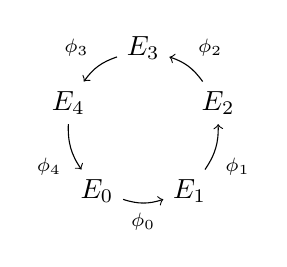
\begin{tikzpicture}
    \def\n{4}
    \foreach \i in {0,...,\n} {
      \pgfmathparse{360/(\n+1)*(\i-1/2) - 90}
      \let\angle\pgfmathresult
      \draw (\angle:1) node (E\i) {$E_\i$};
      % \draw (\angle:0.4) node {\scriptsize$H_\i$};
      % \draw (\angle:0.7) node[rotate=\angle] {\scriptsize$\subset$};
    }
    \foreach \i in {0,...,\n} {
      \pgfmathparse{int(mod(\i+1, \n+1))}
      \let\j\pgfmathresult
      \draw (E\i) edge[->,bend right=18] node[auto,swap] {\scriptsize$\phi_\i$} (E\j);
    }
  \end{tikzpicture}
  \caption{An $\ell$-isogeny volcano with the Vélu isogenies
    represented.}
  \label{fig:volcano}
\end{figure}

Let $\ell$ be a prime different from $p$ and not dividing $q-1$. Let
$E_0$ be an elliptic curve whose cardinality is a multiple of
$\ell$. By Hasse's bound, this is only possible if $\ell\le q +
2\sqrt{q} + 1$. An \emph{isogeny} is an algebraic group morphism
between two elliptic curves that is surjective in the algebraic
closure; it is said to be rational over $\F_q$ if it is invariant
under the $q$-th power map. A rational isogeny between two curves
exists if and only if they have the same number of points over
$\F_q$. The degree of an isogeny is its degree as an algebraic map; an
isogeny of degree $n$ is separable if and only if $n$ is prime to $p$,
in which case its kernel contains exactly $n$ points. A connected
component of the graph whose vertices are elliptic curves up to
isomorphism and whose edges are rational isogenies of degree $\ell$ is
called an \emph{$\ell$-isogeny
  volcano}~\cite{kohel,fouquet+morain02}. It is an undirected graph
and, in the specific case at hand, it is a cycle.
Figure~\ref{fig:volcano} shows one such example with one direction
highlighted. From now on, we denote by $E_0,E_1,\dots$ the curves in
the same volcano as $E_0$.

We now make precise the order in which the curves $E_i$ are
labeled. Suppose that $p\ne2,3$ and let $E_0$ be expressed as the
locus
\begin{equation}
  E_0 \;:\; y^2 = x^3 + ax + b,
  \quad\text{with $a,b\in\F_q$},
\end{equation}
plus one point at infinity. Under the former assumptions on $\ell$,
there exists $e\ge1$ such that the $\ell$-Sylow subgroups of
$E_i/\F_q$ are isomorphic to $\Z/\ell^e\Z$ for any $i$. We denote by
$H_0$ the unique subgroup of $E_0/\F_q$ of order $\ell$, and by
$\phi_0$ the unique isogeny whose kernel is $H_0$; we then label $E_1$
the image curve of $\phi_0$. We go on denoting by $H_i$ the unique
subgroup of $E_i/\F_q$ of order $\ell$, and by $\phi_i:E_i\to E_{i+1}$
the unique isogeny with kernel $H_i$, until we get back to the
starting point.

Vélu's formulas~\cite{velu71} allow us to express the isogenies
$\phi_i$ as rational fractions
\begin{equation}
  \begin{aligned}
    \phi_i: E_i &\to E_{i+1},\\
    (x,y) &\mapsto \left(\frac{f_i(x)}{g_i(x)}, y\left(\frac{f_i(x)}{g_i(x)}\right)'\right),
  \end{aligned}
\end{equation}
where $g_i$ is the square polynomial of degree $\ell-1$ vanishing on
the abscissas of the affine points of $H_i$, and $f_i$ is a polynomial
of degree $\ell$. Algorithmically, Vélu isogenies can be computed
using $O(\Mult(\ell))$ operations in $\F_q$. 

In what follows, the index $i$ in $\phi_i$, $f_i$, $g_i$ and $E_i$ is
to be understood modulo the length of the cycle. This is a slight
abuse, because of some subtleties linked to Vélu's formulas and the
way we consider curves up to isomorphism, but it does not hide any
theoretical or computational difficulty.  For an arbitrary $i$, let
$P$ be a point on $E_{i+1}$ of order divisible by $\ell^e$, Couveignes
and Lercier show that its fiber by $\phi_i$ is irreducible of
cardinality $\ell$. If the order of $P$ is not $2$, all the abscissas
of its fiber are distinct; hence, if $\eta$ is the abscissa of $P$,
the polynomial
\begin{equation}
  \label{eq:isog-fiber}
  f_i(X) - g_i(X)\eta
\end{equation}
is irreducible of degree $\ell$. They also show that, under the same
assumption on $\eta$, the system of equations
\begin{equation}
  \label{eq:elliptic}
  \left|
  \begin{aligned}
    \textstyle
    \frac{f_{i-j}}{g_{i-j}}(X_{j+1}) = X_j\quad\\
    \vdots\qquad\\
    \textstyle
    \frac{f_{i-1}}{g_{i-1}}(X_2) &= X_1\\
              &\textstyle\frac{f_i}{g_i}(X_1) &= \eta
  \end{aligned}
  \right.
\end{equation}
defines an $\ell$-adic closure of $\F_q$. By composing the relations,
we have that
\begin{equation}
  \label{eq:elliptic-uni}
  \frac{f_i}{g_i}\left(\frac{f_{i-1}}{g_{i-1}}\left(\cdots\frac{f_{i-j}}{g_{i-j}}(X)\right)\right) = \eta
\end{equation}
defines an extension of $\F_q$ of degree $\ell^{j+1}$. In the next
section we show how to compute this relation efficiently.

\begin{remark}
  \label{rk:cycle}
  There is a major difference between our setting and Couveignes' and
  Lercier's. Observe that, once a point $P$ of $E_i$ is chosen, the
  $\ell$-adic tower is constructed by walking \emph{backwards} in the
  isogeny cycle. The goal of~\cite{couveignes+lercier11}, is to
  compute an extension of degree $\ell^i$ of $\F_q$ for a certain
  fixed $i$. Under the former assumptions, using the construction we
  just presented this can be done in quasi-linear time in $\ell^i$:
  apply $i$ times Vélu's formulas, then take the fiber of a point of
  $E_i$ by the isogenies $\phi_{i-1}, \ldots, \phi_0$. In our case, we
  are interested in building extensions of degree $\ell^i$
  \emph{incrementally}, i.e.\ without any \emph{a priori} bound on
  $i$. We have two ways of doing this:
  \begin{enumerate}
  \item Precompute the whole cycle, this can be done using Vélu's
    formulas only. Assuming the cycle has length $n$, chose a point of
    $E_0$ and take its fiber by the isogenies $\phi_{n-1}, \ldots,
    \phi_0, \phi_{n-1}, \ldots$ The length of the isogeny cycle is the
    order of a certain ideal in the class group of the endomorphism
    ring of $E_0$, thus it is proportional to $\sqrt{q}$. Hence, this
    approach has a quasi-linear complexity in $\ell^i$, but an
    exponential complexity in $\log q$.
  \item Compute the curves on the isogeny cycle backwards, then apply
    Vélu's formulas. This can be done incrementally, thus it does not
    require to precompute the whole isogeny cycle. However, computing
    $E_{i-1}$ from the knowledge of $E_i$ can only be done by
    factoring the $\ell$-th \emph{modular polynomial}~\cite{schoof95},
    a task requiring $O(\ell^3)$ bit operations and $O(\ell^2)$
    operations in $\F_q$~\cite{sutherland10:modpol}.
  \end{enumerate}
\end{remark}

%%%

\section{Lifting and pushing}
\label{sec:lift-push}

Until now we have shown how to compute some systems of irreducible
polynomials defining an $\ell$-adic closure of $\F_q$, but we have not
explained how to represent the elements of $\F_q^{(\ell)}$ and how to
perform asymptotically fast arithmetic. For simplicity we will only
address the construction of $\F_p^{(\ell)}$. Adapting it to
$\F_q^{(\ell)}$ only requires bivariate arithmetic and presents no
major difficulty.

We follow the same paradigm as in~\cite{df+schost12}. Each of the
finite subfields $\F_{p^{\ell^i}}$ of $\F_p^{(\ell)}$ is represented
as a univariate quotient ring $\F_p[X_i]/P_i(X_i)$. This allows for
asymptotically fast multiplication and inversion of elements of
$\F_{p^{\ell^i}}$. Elements of $\F_p^{(\ell)}$ are represented as
elements of the smallest subfield containing them. Operations between
elements of different subfields are performed by \emph{lifting} the
element of the smallest subfield into the largest one. An inverse
operation, called \emph{push}, is also needed in order to cast,
whenever possible, elements of a larger subfield into a smaller one.

The lift and push operations need only be described between a pair
$\F_{p^{\ell^{i-1}}}$, $\F_{p^{\ell^i}}$ of consecutive levels in the
$\ell$-adic tower. Any other pushing and lifting is done by applying
repeatedly these elementary operations. According to
Eqs.~\eqref{eq:T1}, \eqref{eq:T2-relpols} and~\eqref{eq:elliptic}, all
the constructions of the previous sections fit in the same pattern:
$\F_{p^{\ell^{i-1}}}$ is generated over $\F_p$ by an element $x$ such
that
\begin{equation}
  \label{eq:level-i}
  \frac{F(x)}{G(x)} = \eta,
\end{equation}
where $F$ is a polynomial of degree $\ell^{i-1}$, $G$ is a polynomial
of degree less than $\ell^{i-1}$ (eventually, $G=1$), and $\eta$ is an
element of $\F_p$. In its turn, $\F_{p^{\ell^i}}$ is generated over
$\F_p$ by an element $y$ such that
\begin{equation}
  \label{eq:level-i+1}
  \frac{f(y)}{g(y)} = x,
\end{equation}
where $f$ is a polynomial of degree $\ell$, and $g$ is a
polynomial of degree less than $\ell$ (eventually, $g=1$). The
minimal polynomial of $y$ over $\F_p$ is obtained by composing
Eqs.~\eqref{eq:level-i} and~\eqref{eq:level-i+1}:
\begin{equation}
  \label{eq:minpol-compose}
  \frac{F}{G}\left(\frac{f}{g}(y)\right) = \eta.
\end{equation}

\begin{corollary}
  \sloppy
  Let $y$ be the generator of $\F_{p^{\ell^i}}$ over
  $\F_{p^{\ell^{i-1}}}$. Its minimal polynomial over $\F_p$ can be
  computed using $O(\Mult(\ell^i)\log\ell^i)$ operations in $k$.
\end{corollary}
\begin{proof}
  Remark that for $T_1$ and $T_2$-type extension we have more
  efficient ways of computing these polynomials. In the general case,
  the composition in Eq.~\eqref{eq:minpol-compose} can be computed
  using Algorithm~\ref{alg:compose}. The complexity bound is proved in
  Theorem~\ref{th:compose}.
\end{proof}

In view of this, there are two natural ways to represent elements of
$\F_{p^{\ell^i}}$: as univariate polynomials in $y$, or as bivariate
polynomials in $x$.

\begin{definition}
  Let $x$ and $y$ be as above, we define the two following
  $\F_p$-vector space bases of $\F_{p^{\ell^i}}$.
  \begin{align}
    \label{eq:uni-basis}
    \uu &= \left(y^j \;\middle|\; 0\le j <\ell^i\right),\\
    \label{eq:bi-basis}
    \bb &= \left(y^jx^k \;\middle|\; 0\le j <\ell, 0\le k <\ell^{i-1}\right).
  \end{align}
\end{definition}

We call \emph{lifting} the conversion of an element from $\bb$ to
$\uu$, \emph{pushing} the inverse transformation. We now present
algorithms to perform each of them.

\paragraph{Lifting}
We are faced with the following problem. We have polynomials $P$, $f$
and $g$ with coefficients in a field $k$, and we want to compute the
composition $P(f/g)$.

\begin{definition}
  Let $P,f,g$ be polynomials, we denote by $P[f,g]$ the numerator of
  $P(f/g)$, so that
  \begin{equation}
    P\left(\frac{f}{g}\right) = \frac{g^nP(f/g)}{g^n} = \frac{P[f,g]}{g^n}.
  \end{equation}
  If $P=\sum_0^np_iX^i$, then
  \begin{equation}
    P[f,g] = \sum_{i=0}^n  p_if^ig^{n-i}.
  \end{equation}
\end{definition}

\begin{algorithm}[t]
  \caption{Compose}
  \label{alg:compose}
  \begin{algorithmic}[1]
    \REQUIRE $P\in k[Y][X]$, $f,g\in k[Y]$;
    \STATE $n \la \deg_X P$;
    \IF {$n = 0$}
    \ENSURE $P$
    \ELSE
    \STATE $m \la \lceil n/2\rceil$;
    \STATE Let $P_0,P_1$ be such that $P = P_0 + X^mP_1$;
    \STATE $Q_0 \la$ Compose($P_0, f, g$);
    \STATE $Q_1 \la$ Compose($P_1, f, g$);
    \STATE \label{alg:compose:res}
    $Q \la Q_0g^{n-m+1} + Q_1f^m$;
    \ENSURE $Q$.
    \ENDIF
  \end{algorithmic}
\end{algorithm}

\begin{theorem}
  \label{th:compose}
  On input $P,f,g$, Algorithm~\ref{alg:compose} computes the
  polynomial $P[f,g]$. If $n=\deg_XP$, $\ell=\max(\deg f, \deg g)$ and
  $\deg_YP\in O(\ell)$, it computes its output using $O(\Mult(\ell
  n)\log n)$ operations in $k$.
\end{theorem}
\begin{proof}
  If $n=0$, the theorem is obvious. Suppose $n>0$, then $P_0$ and
  $P_1$ have degree $m-1$ and $n-m$ respectively. By induction
  hypothesis,
  \begin{equation}
    \begin{aligned}
      Q_0 &= P_0[f,g] = \sum_{i=0}^{m-1}p_if^ig^{m-1-i},\\
      Q_1 &= P_1[f,g] = \sum_{i=0}^{n-m}p_{i+m}f^ig^{n-m-i}.   
    \end{aligned}
  \end{equation}
  Hence,
  \begin{equation}
    Q = \sum_{i=0}^{m-1}p_if^ig^{n-i} +
    \sum_{i=0}^{n-m}p_{i+m}f^{i+m}g^{n-m-i} =
    P[f,g].
  \end{equation}

  The only step that requires a computation is
  Step~\ref{alg:compose:res}, costing $O(\Mult(\ell n))$ operations in
  $k$. The recursion has depth $\log n$, hence the overall complexity
  is $O(\Mult(\ell n)\log n)$.  Observe that when $g=1$,
  Algorithm~\ref{alg:compose} reduces to a well known algorithm for
  polynomial composition~\cite[Ex.~9.20]{vzGG}.
\end{proof}

\begin{corollary}
  Let $\alpha\in\F_{p^{\ell^i}}$ be represented on the basis $\bb$.
  We can \emph{lift} $\alpha$ to the basis $\uu$ using
  $O(\Mult(\ell^i)\log\ell^i)$ operations in $\F_p$.
\end{corollary}
\begin{proof}
  $\alpha$ is represented by a bivariate polynomial $P(y,x)$ with
  $\deg_yP<\ell$ and $\deg_xP<\ell^{i-1}$.  We compute the univariate
  polynomials $P[f,g]$ and $g^n$, using $O(\Mult(\ell^i)\log\ell^i)$
  operations in $\F_p$. We interpret $P[f,g](y)$ and $g^n(y)$ as
  elements of $\F_{p^{\ell^i}}$ written in the basis $\uu$. Then the
  lift of $\alpha$ is $P[f,g](y)/g^n(y)$. The inversion of $g^n(y)$
  can be computed in $O(\Mult(\ell^i)\log\ell^i)$ using the extended
  Euclidean algorithm.
\end{proof}

\paragraph{Pushing}
We now have the inverse problem. We are given polynomials $P$, $f$ and
$g$, with coefficients in a field $k$, and such that $(f,g)=1$. Using
the same notation as before, we want to compute a decomposition
$P=Q[f,g]$.

\begin{algorithm}[t]
  \caption{Decompose}
  \label{alg:decompose}
  \begin{algorithmic}[1]
    \REQUIRE $P,f,g\in k[Y]$ s.t. $\deg g<\deg f$ and $(f,g)=1$;
    \REQUIRE $n\in\N$;
    \IF {$n=0$}
    \ENSURE $P$
    \ELSE
    \STATE $m \la \lceil n/2 \rceil$;
    \STATE \label{alg:decompose:xgcd}
    Compute $u, v$ such that $uf^m + vg^m = 1$;
    \STATE $r \la 0$;
    \IF {$\deg P \ge \deg f^m + \deg g^m$}
    \STATE \label{alg:decompose:div}
    $q,\; P \la P \div f^m,\; P \bmod f^m$;
    \ENDIF
    \STATE \label{alg:decompose:split}
    $P_0,\; P_1 \la Pv \bmod f^m,\; q + (Pu \bmod g^m)$;
    \STATE $Q_0 \la$ Decompose($P_0, f, g, n-m$);
    \STATE $Q_1 \la$ Decompose($P_1, f, g, n-m$);
    \ENSURE $Q_0 + X^mQ_1$.
    \ENDIF
  \end{algorithmic}
\end{algorithm}

\begin{theorem}
  On input $P,f,g,n$, Algorithm~\ref{alg:decompose} computes a
  polynomial $Q\in k[Y][X]$ such that $\deg_X Q=n$ and $P=Q[f,g]$.

  Let $\ell=\deg f$. If $\deg P < \ell(n+1)$, then $\deg_Y Q<\ell$. In
  this case, the output is computed using $O(\Mult(\ell n)\log \ell
  n)$ operations in $k$.
\end{theorem}
\begin{proof}
  If $n=0$ the statement is obvious. In particular, if $\deg P <
  \ell$, the output trivially satisfies $\deg_YQ<\ell$.

  Let $n>0$, then $m>0$. We prove the theorem by induction. The
  polynomials $P_0$ and $P_1$ computed in
  Step~\ref{alg:decompose:split} verify
  \begin{equation}
    \begin{aligned}
      P &\equiv P_0g^m \mod f^m,\\
      P &\equiv P_1f^m \mod g^m.
    \end{aligned}
  \end{equation}
  Comparing degrees and using the Chinese remainder theorem, we
  conclude that
  \begin{equation}
    P = P_0g^m + P_1f^m.
  \end{equation}
  We necessarily have $n-m<n$, hence, by induction hypothesis, $Q_0$
  and $Q_1$ have degree $n-m$ and are such that
  \begin{equation}
    \begin{aligned}
      P_0 &= Q_0[f,g] = \sum_{i=0}^{n-m} q_{0,i}f^ig^{n-m-i},\\
      P_1 &= Q_1[f,g] = \sum_{i=0}^{n-m} q_{1,i}f^ig^{n-m-i}.
    \end{aligned}
  \end{equation}
  Hence, $Q=Q_0+X^mQ_1$ has degree $n$ and is such that
  \begin{multline}
    Q[f,g] = \sum_{i=0}^{n-m}q_{0,i}f^ig^{n-i} + 
    \sum_{i=m}^nq_{1,i-m}f^ig^{n-i} =\\
    Q_0[f,g]g^m + Q_1[f,g]f^m = P.
  \end{multline}

  If $\deg P < \ell (n+1)$, both $P_0$ and $P_1$ have degree less than
  $\ell(n-m+1)$. Then, by induction hypothesis, $\deg q_{0,i}<\ell$
  and $\deg q_{1,i}<\ell$ for any $i$. We deduce that
  $\deg_YQ<\ell$. Observe that when $g=1$,
  Algorithm~\ref{alg:decompose} reduces to Algorithm~9.14
  of~\cite{vzGG}.

  Finally we analyze the complexity of the algorithm on input $P, f,
  g, n$, under the constraints on the degrees specified
  above. Step~\ref{alg:decompose:xgcd} is dominated by the extended
  Euclidean algorithm, which costs $O(\Mult(\ell n)\log \ell n)$
  operations in $k$. Although Algorithm~\ref{alg:decompose} is
  recursive, this step is independent of $P$, thus it can be done just
  once for every $m$, before running the rest of the algorithm. The
  dominant cost is the one of the highest power $m$, contributing
  $O(\Mult(\ell n)\log \ell n)$ to the overall complexity. This
  precomputation saves a logarithmic factor.

  We are left with the contribution of Steps~\ref{alg:decompose:div}
  and~\ref{alg:decompose:split}, costing $O(\Mult(\ell n))$ each. The
  recursion has depth $\log n$, thus the overall cost is $O(\Mult(\ell
  n)\log n)$. Hence, the total complexity is dominated by the cost of
  Step~\ref{alg:decompose:xgcd}.
\end{proof}

\begin{corollary}
  Let $\alpha\in\F_{p^{\ell^i}}$ be represented on the basis $\uu$. We
  can \emph{push} $\alpha$ to the basis $\bb$ using
  $O(\Mult(\ell^i)\log\ell^i)$ operations in $\F_p$.
\end{corollary}
\begin{proof}
  $\alpha$ is represented by a univariate polynomial $P(y)$ of degree
  less than $\ell^i$. We compute $g^{\ell^{i-1}-1}$ and $\bar{P}(y) =
  g^{\ell^{i-1}-1}(y)P(y)$ using $O(\Mult(\ell^i))$ operations. Then,
  we apply Algorithm~\ref{alg:decompose} to $\bar{P}$, $f$ and $g$,
  with $n=\ell^{i-1}-1$. The result is a bivariate polynomial $Q$,
  representing $\alpha$ on the basis $\mathbf{B}$. The dominant phase
  is Algorithm~\ref{alg:decompose}, costing
  $O(\Mult(\ell^i)\log\ell^i))$ operations in $\F_p$.
\end{proof}

%%%

\section{Implementation}
\label{sec:impl}

Sage implementation and timings.

%%%

\section{Aknowledgements}
De Feo would like to thank Antoine Joux.

\scriptsize
\bibliographystyle{abbrv}
\bibliography{defeo}
\end{document}


% Local Variables:
% mode:flyspell
% ispell-local-dictionary:"american"
% mode:TeX-PDF
% mode:reftex
% End:
%
% LocalWords:  Isogeny abelian isogenies hyperelliptic supersingular Frobenius
% LocalWords:  isogenous embeddings Vélu




